\documentclass[../main.tex]{subfiles}





\begin{document}






\chapter{Políedres}


En aquest capítol es formalitza el concepte de políedre simplicial, que correspon a un subespai de $\mathbb{R}^N$ construït a partir de símplexs, enganxats de forma convenient. Aquests espais estan a la base de les tècniques d'homologia que desenvoluparem en els capítols següents.

Els políedres simplicials són, per la seva pròpia definició, subespais d'un espai afí $\mathbb{R}^N$ i per a ells cal especificar els diferents símplexs que el componen.


\section{Símplexs i políedres simplicials}

Els políedres que anem a introduir en aquest apartat són espais topològics construïts a partir de símplexs. Començarem la secció a través del que anomenarem complex simplicial, que és el conjunt de símplexs que el formen.

En tot el que segueix, $\mathbb{R}^N$ denotarà l'espai afí euclidià de dimensió $N$ amb la topologia induïda per la distància euclidiana, és a dir, la definida per $d(x,y) = \|x-y\|$ per a tot parell de punts $x,y\in\mathbb{R}^N$.

Comencem fent un recordatori de la noció de conjunt convex:

\begin{defi}[Convex]\index{Convex}
Si $C\subset\mathbb{R}^N$, diem que $C$ és \textit{complex} si per a tota parella $p,q\in C$, $\forall t\in[0,1]$ es compleix que $tp+(1-t)q\in C$. És a dir, que per a tota parella de punts, el segment que els uneix està completament a dins de $C$.
\end{defi}

Definim el nostre ``producte essencial'' de la secció, el $n$-símplex o símples $n$-dimensional.

\begin{defi}[$n$-símplex]\index{$n$-símplex}\index{Símplex}
Siguin $v_0,\ldots,v_n\in\mathbb{R}^N$ tals que $v_1-v_0,\ldots,v_n-v_0$ són linealment independents, anomenarem \textit{$n$-símplex} determinat per $v_0,\ldots,v_n$ al més petit subconjunt convex de $\mathbb{R}^N$ que conté $v_0,\ldots,v_n$. El denotarem $\langle v_0,\ldots,v_n\rangle$. En aquest context, es diu que $v_0,\ldots,v_n$ són els \textit{vèrtexs} de $\langle v_0,\ldots,v_n\rangle$.\index{Vèrtex d'un símplex}
\end{defi}


\begin{nota}
Té sentit parlar del ``més petit convex'' perquè és fàcil demostrar que la intersecció de convexos és convex.
\end{nota}




\begin{defi}
\label{def:simplexestandard}\index{Símplex estàndard} El $n$-\textit{símplex estàndard}\index{$n$-símplex estàndard} és
\begin{equation}
    \notag
    \Delta^n = \left\{(t_0,\ldots,t_n)\in\mathbb{R}^{n+1}\;:\;t_i\geq 0,\;\sum_{i=0}^n t_i = 1\right\} = \langle \mathbf{e}_1,\ldots,\mathbf{e}_n\rangle
\end{equation}
on $\mathbf{e}_i = (0,\ldots,0,1,0,\ldots,0)$ i l'1 està en la posició $i$-ésima. Com a exemples concrets, $\Delta^1$ és un segment en el pla, $\Delta^2$ és un triangle en $\mathbb{R}^3$.
\end{defi}

\begin{ej}
Fem exemples de $\Delta^n$. Si $n = 0$, el $\Delta^0$ és un punt, si $n = 1$ tenim $\Delta^1$ igual a un segment, si $n = 2$ tenim $\Delta^2$ igual a un triangle, si $n = 3$ un tetraedre, etc.
\begin{equation}
    \notag
    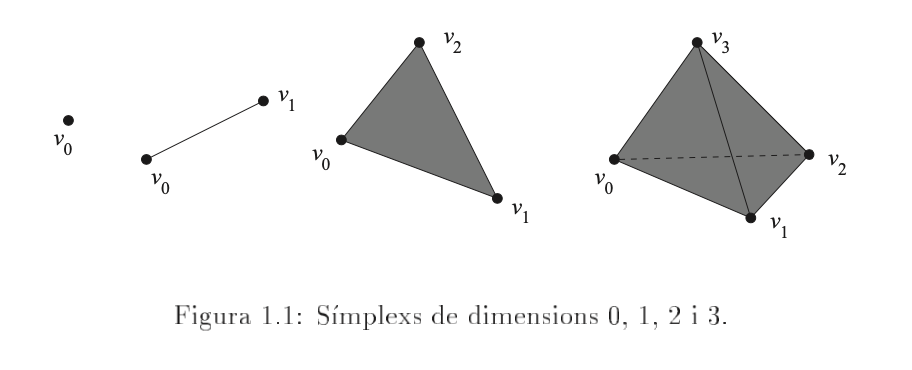
\includegraphics[scale = 0.5]{pictures/exemplesnsimplex.png}
\end{equation}
\end{ej}

Tot símplex és un subconjunt de $\mathbb{R}^N$, i és per tant un espai topològic amb la topologia induïda per la de $\mathbb{R}^N$.


\begin{lema}
\begin{enumerate}[(i)]
    \item Tot $n$-símplex és homeomorf al $n$-símplex estàndard.
    \item Tot $n$-símplex és compacte, connex, localment arc-connex i contràctil.
\end{enumerate}
\end{lema}
\begin{proof}
Es deixa com a exercici pel lector o lectora.
\end{proof}

\begin{defi}
\index{Cares $k$-dimensionals} Sigui $\langle v_1,\ldots,v_n\rangle$ un $n$-símplex. Anomenem cares $k$-dimensionals de $\langle v_0,\ldots,v_n\rangle$ als símplexs $\langle v_{i_0},\ldots,v_{i_k}\rangle$ amb $0\leq i_0<i_1<\cdots<i_k\leq n$. A les cares de dimensió 1 se les sol anomenar arestes.
\end{defi}

Per exemple, en $\Delta^2$, que és un triangle, les arestes són cares 1-dimensionals i els vèrtexs són cares 0-dimensionals. Tot el triangle seria una cara 2-dimensional.

\begin{defi}
[Complex simplicial]\label{def:complexsimplicial}\index{Complex simplicial} Un \textit{complex simplicial} és un conjunt finit de símplexs de $\mathbb{R}^N$, $K=\{\sigma_1,\ldots,\sigma_r\}$ tals que
\begin{enumerate}[(i)]
    \item Si $\sigma_i$ és un símplex de $K$, aleshores totes les cares de $\sigma_i$ són de $K$.
    \item Si $\sigma_i$ i $\sigma_j$ són símplexs de $K$, aleshores $\sigma_i\cap\sigma_j\not=\emptyset$ o bé $\sigma_i\cap\sigma_j$ és una cara de $\sigma_i$ i de $\sigma_j$.
\end{enumerate}
\end{defi}

Per simplificar l'exposició, considerarem únicament políedres formats per un nombre finit de símplexs, com en la definició anterior. És possible, però, definir políedres construïts a partir d'un nombre infinit de símplexs. En aquest cas, cal demanar alguna altra propietat a més de les dues de la definició, que eviti, per exemple, considerar $\mathbb{R}$ com un políedre de dimensió zero degut a l'agregació d'infinits $0$-símplexs, un per cada punt de $\mathbb{R}$, el que entraria en contradicció amb la noció intuïtiva de dimensió, i que més endavant formalitzarem. Ara però, pel que ens ocupa, no és necessari detallar la definició de complex simplicial infinit.


\begin{defi}
[Políedre geomètric]\label{def:poliedregeometric}\index{Políedre geomètric} Donat un complex simplicial $K$, s'anomena \textit{políedre geomètric associat a $K$}\footnote{Els políedres simplicials són espais topològics fàcilment visualitzables i suficientment generals com per tenir aplicacions significatives. La definició que hem donat es deu a Henri Poincaré, qui va adonar-se de les bones propietats d'aquests espais i els va introduir al voltant de l'any 1899.}, al subespai de $\mathbb{R}^N$
\begin{equation}
    \notag
    |K| = \bigcup_{\sigma\in K}\sigma,
\end{equation}
és a dir, al subespai de $\mathbb{R}^N$ definit per la reunió de tots els símplexs de $K$. Si $P = |K|$, es diu que $P$ és una triangulació de $K$.
\end{defi}

Observem que, per un determinat símplex, el seu políedre geomètric és ell mateix, i.e. $|\sigma| = \sigma$, per $\sigma$ símplex. Vegem ara uns altres exemples.

\begin{ej}
\label{ej:poliedregeometric} 
\begin{enumerate}[(a)]
    \item El símplex $\Delta^n$ determina un políedre geomètric.
    \item La vora de $\Delta^{n+1}$, que denotarem $\partial\Delta^{n+1}$ és el complex simplicial que està format per les cares de dimensió $\leq n$ de $\Delta^{n+1}$.
\end{enumerate}
\end{ej}


\begin{nota}
Es dona el següent homeomorfisme: $|\partial\Delta^{n+1}|\simeq \mathbb{S}^n$.
\end{nota}
\begin{proof}
Exercici.
\end{proof}

\begin{nota}\label{nota:poliedresgeometrics}
Fem alguns apunts interessants sobre els políedres geomètrics. Suposem $K$ un complex simplicial.
\begin{enumerate}[(1)]
    \item $|K|$ és compacte, localment arc-connex i localment contràctil.
    \item Si $X$ és un espai topològic, considerem $f:|K|\rightarrow X$ una aplicació. Aleshores, $f$ és contínua si, i només si, $\forall \sigma\in K$, $f_{|\sigma}$ és contínua.
\end{enumerate}
\end{nota}


\begin{coro}
Sigui $K$ un complex simplicial, $X$ un espai topològic i $f:|K|\rightarrow X$ una aplicació. Aleshores $f$ és contínua si, i només si, ho és cadascuna de les restriccions $f_{|\sigma}$ a cada símplex $\sigma$ de $K$.
\end{coro}

Un dels avantatges que presenten els políedres respecte dels espais topològics en general és que pot introduir-se un concepte de dimensió de manera natural.

Sigui $K$ un complex simplicial. Direm que $K$ és un complex simplicial de dimensió $n$, o que el políedre $|K|$ és de dimensió $n$, si $n$ és la més gran de les dimensions de les cares de $K$.

\begin{defi}
[Conjunt de les cares]\index{Conjunt de les cares}\index{$C_p(K)$} Notarem $C_p(K)$ el conjunt de les cares $p$-dimensionals de $K$ i $c_p$ el nombre de cares $p$-dimensionals de $K$, i.e. $c_p:=\#C_p(K)$. 
\end{defi}

Exemples ben senzills mostren que $c_p$ no són invariants topològics d'un políedre. Per exemple, tots els polígons regulars d'$n$ costats, $P_n$, són homeomorfs, mentre que $c_0(P_n) = n$ i $c_1(P_n) = n$, varien en funció de $n$.

\begin{defi}
[Característica d'Euler]\index{Característica d'Euler} Sigui $K$ un complex simplicial. Es defineix la \textit{característica d'Euler}\footnote{També coneguda com a característica d'Euler-Poincaré} de $K$ com la suma alternada
\begin{equation}
    \notag
    \chi(K) = \sum_{i\geq 0}(-1)^{i}c_i = c_0-c_1+c_2-\cdots
\end{equation}
\end{defi}

Com que els políedres que considerem són sempre finits, la suma que defineix la característica d'Euler és un enter finit, i.e. per tot $K$ complex simplicial finit, $\chi(K)\in\mathbb{Z}$.

\begin{ej}
\begin{enumerate}[(a)]
    \item Sigui $K$ el complex simplicial que correspon a una triangulació de la superfície d'un cub com la indicada a la figura \ref{fig:triangulaciodelasuperficieduncub}. Aleshores, $\chi(K) = 8-18+12=2$.
    \begin{figure}
        \centering
        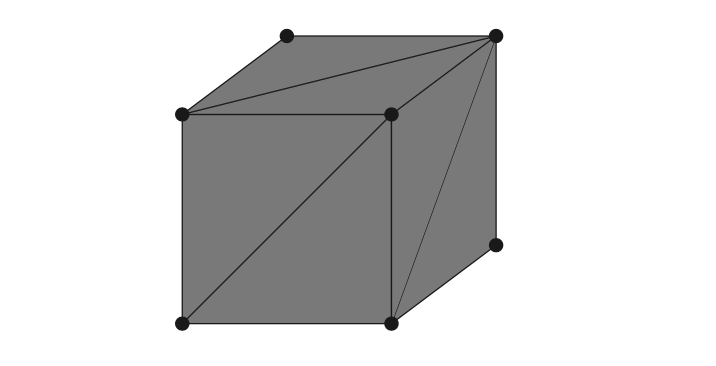
\includegraphics[scale = 0.5]{pictures/cubtriangulat.png}
        \caption{Triangulació de la superfície d'un cub}
        \label{fig:triangulaciodelasuperficieduncub}
    \end{figure}
    \item La característica d'Euler d'un símplex $n$-dimensional estàndard, $\Delta^n$, és $\chi(\Delta^n) = 1$. En efecte, $\Delta^n$ té $n+1$ vèrtexs i les cares $p$-dimensionals corresponen a totes les eleccions possibles de $p+1$ vèrtexs diferents, per tant es té
    \begin{equation}
        \notag
        c_p(\Delta^n) = \binom{n+1}{p+1}
    \end{equation}
    i, en definitiva,
    \begin{equation}
        \notag
        \chi(\Delta^n) = \binom{n+1}{1}-\binom{n+1}{2}+\cdots+(-1)^n\binom{n+1}{n+1} = 1
    \end{equation}
    \item La característica d'Euler de la vora de $\Delta^n$, i.e. $\partial \Delta^n$, és
    \begin{equation}
        \notag
        \chi(\partial\Delta^n) = 1-(-1)^n = 1+(-1)^{n-1}
    \end{equation}
\end{enumerate}
\end{ej}

En els exemples anteriors hem vist que, tant la característica d'Euler de la superfície d'un cub com la de $\partial\Delta^3$ són iguals a 2. Aquests dos espais són homeomorfs, cosa que ens porta a plantejar-nos la següent pregunta natural: són la dimensió i la característica d'Euler invariants topològics? És a dir, si $K$ i $L$ són complexos simplicials tals que els políedres associats, $|K|$ i $|L|$ respectivament, són espais homeomorfs, és cert que la dimensió i la característica d'Euler de $K$ i $L$ són iguals?

Més endavant provarem que la resposta és afirmativa i que, fins i tot, la característica d'Euler és un invariant d'homotopia. En particular, per exemple, en resultarà que $\partial\Delta^2$ i $\partial\Delta^3$ són homotòpicament equivalents.


\section{Aplicacions simplicials}

Per a què la noció d'espai topològic sigui d'utilitat és essencial disposar de la noció d'aplicació contínua entre espais topològics, de forma que es tingui una categoria, la categoria d'espais topològics $\mathbf{Top}$. En el context simplicial, la noció corresponent és la d'aplicació simplicial.

\begin{defi}[Aplicació simplicial]\index{Aplicació simplicial}
Siguin $K$ i $L$ complexos simplicials, siguin $V_k$ i $V_L$ els (conjunts de) vèrtexs de $K$ i $L$. Sigui $\varphi_0:V_K\rightarrow V_L$ tal que si $\{p_0,\ldots,p_r\}\subset V_K$ determinen un símplex de $K$, aleshores $\{\varphi_0(p_0),\ldots,\varphi_0(p_r)\}$ determina un símplex en $L$. Podem definir
\begin{equation}
    \notag
    \begin{array}{rl}
        \varphi:K & \longrightarrow L \\
        \sigma & \varphi(\sigma)
    \end{array}
\end{equation}
on $\varphi(\sigma)$ es diu \textit{envolvent connexa de $\{\varphi_0(p_0),\ldots,\varphi_0(p_r)\}$}\index{Envolvent connexa}. Es diu que $\varphi$ és \textit{simplicial}.
\end{defi}


\begin{defi}
Siguin $K,L$ complexos simplicials, sigui $\varphi:K\rightarrow L$ simplicial. Denotarem $|\varphi|$ l'aplicació
\begin{equation}
    \notag
    |\varphi|:|K|\longrightarrow|L|
\end{equation}
tal que si $\sigma= \langle v_0,\ldots,v_p\rangle\in |K|$, aleshores
\begin{equation}
    \notag
    |\varphi|\left(\sum_{i=0}^p\lambda_iv_i\right)=\sum_{i=0}^p\lambda_i\varphi_0(v_i)
\end{equation}
on les $\lambda_i$ són les \textit{coordenades baricèntriques}\index{Coordenades baricèntriques} en $\sigma$.
\end{defi}


\begin{defi}[Lineal a trossos]
Si $P$ i $Q$ són políedres geomètrics i $f:P\rightarrow Q$ una aplicació, es diu que $f$ és \textit{lineal a trossos}\index{Lineal a trossos}\index{Lineal a peces} (o a peces) si existeixen complexos simplicials $K$ i $L$ tals que $P = |K|$, $Q = |L|$, existeix $\varphi:K\rightarrow L$ simplicial tal que $f =|\varphi|$.
\end{defi}

\begin{nota}
Els complexos simplicials formen una categoria i
\begin{equation}
    \notag
    |\bullet|:\mathrm{CompSim}\rightarrow\mathrm{Top}
\end{equation}
és un functor.
\end{nota}


\begin{defi}
[Triangulació]\index{Triangulació} Si $X$ és un espai topològic, una \textit{triangulació} de $X$ és $(K,\varphi)$ on $K$ és un complex simplicial i $\varphi:X\rightarrow|K|$ és un homeomorfisme. Direm que $X$ és \textit{triangulable}\index{Triangulable} si admet com a mínim una triangulació.
\end{defi}


\begin{ej}
\begin{enumerate}[(a)]
    \item La bola $\mathbb{B}^n = \{(x_1,\ldots,x_n)\in\mathbb{R}^n\;:\;\sum_{i=1}^n x_i^2\leq 1\}\simeq |\Delta^n|$ és triangulable, ja que és homeomorfa a un $n$-símplex.
    \item L'esfera de dimensió $n$, $\mathbb{S}^n = \{x\in\mathbb{R}^{n+1}\;:\;\|x\|=1\}$, és un espai triangulable ja que és homeomorfa al políedre $\partial\Delta^{n+1}$.
\end{enumerate}
\end{ej}



%%%% C'EST FINI










\end{document}